\begin{problem}{璃月的桥梁}{standard input}{standard output}{1 second}{256 megabytes}

原神中,主角旅行者擅长借助传送锚点进行快速移动,具体地说旅行者可以从任何位置传送到指定传送锚点的位置。

璃月的华光林有几个几乎无法攀爬的极高的山峰,它们之间用一些木桥梁连接。这些山峰中有且仅有一个拥有传送锚点。

\begin{center}
  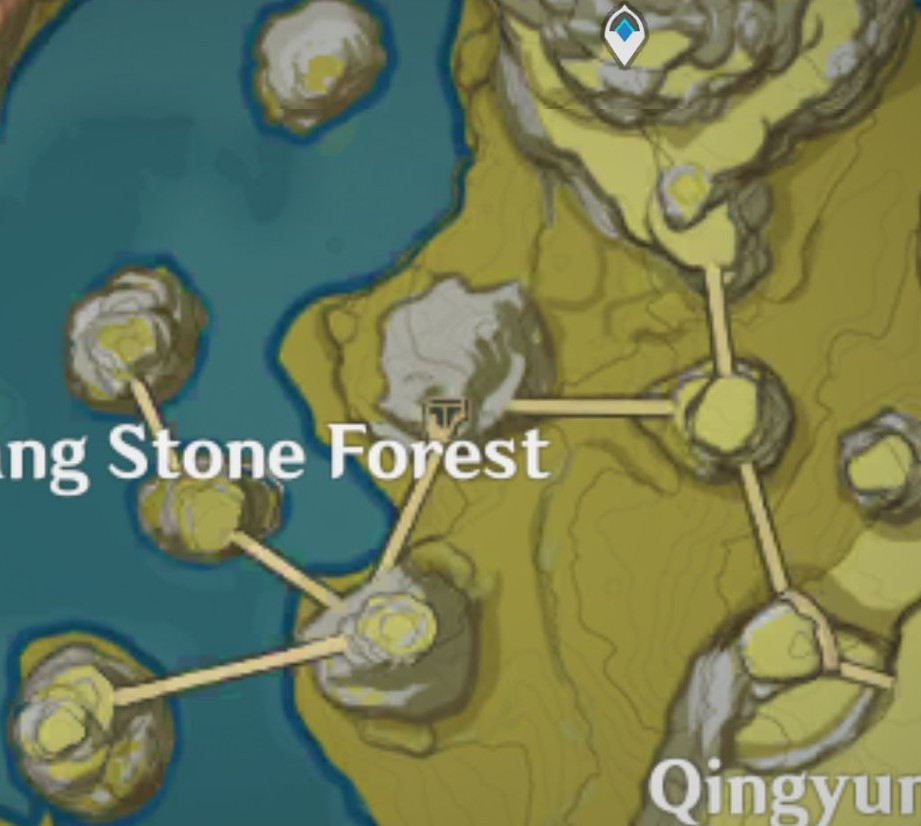
\includegraphics[scale=0.8]{path.jpg} \\
  \small{华光林}
\end{center}

最近,旅行者接到一份委托,要求旅行者去检修这些桥梁,为了使得检修时间最短,旅行者希望找到一条路径,这条路径\textbf{从传送锚点出发},恰好经过每条桥梁一次,\textbf{可以在任意山峰结束}。

你的任务是判断旅行者想要的路径是否存在。

\InputFile
第一行两个整数$n$、$m$,山峰的数量和桥梁的数量,其中令带有传送锚点的山峰为$1$号。($3 \le n \le 200$,$2 \le m \le \dfrac{n(n - 1)}{2}$)

接下来$m$行,每行一个两个整数$u$、$v$,表示一个桥梁连接$u$、$v$两座山峰。($1 \le u < v \le n$)

保证从传送锚点可以到达任意山峰,保证不存在两座桥梁连接相同的两座山峰。

\OutputFile
如果路径存在,输出``YES'',否则输出``NO'',不区分大小写。

\Examples

\begin{example}
\exmpfile{example.01}{example.01.a}%
\exmpfile{example.02}{example.02.a}%
\exmpfile{example.03}{example.03.a}%
\end{example}

\end{problem}

